\chapter{Division II: turning division into multiplication}
\label{ch:fastdiv}

Long division costs (quotient length) $\times$ (divisor length). The methods in this chapter
reduce division to a small number of multiplications, so that division automatically
inherits Karatsuba, Toom-3 and the NTT. There are three ideas:

\begin{description}[leftmargin=2.8cm,style=sameline]
  \item[Burnikel--Ziegler] Do long division, but with each ``digit'' a large block, and the
        block steps done recursively.
  \item[Newton] Compute $1/b$ once, very accurately; then $a/b$ is $a \times (1/b)$ plus a
        small correction.
  \item[Top limbs] When the quotient is short, only the leading limbs of $a$ and $b$ matter.
\end{description}

\section{Burnikel--Ziegler: long division with big digits}
\label{sec:bz}

Go back to the long division of \cref{sec:knuth}, but imagine the ``digits'' are blocks of
many limbs. Each round still guesses a quotient block, multiplies it back, and corrects. The
guessing step is itself a division, of a smaller size, so it can be done by the same method,
recursively. The multiply-back step is a block-by-block multiplication, so it uses the fast
multipliers. This is Christoph Burnikel and Joachim Ziegler's recursive division (1998).

\subsection{One level of the recursion}

Split the normalized divisor into a high and a low half, $d = d_{\text{hi}} X + d_{\text{lo}}$.
To divide a $2n$-limb number by the $n$-limb $d$, compute the quotient in two halves. For each
half:

\begin{enumerate}
  \item Divide the top of the current remainder by $d_{\text{hi}}$ \emph{only}. This is a
        half-size division, done recursively. It gives a quotient guess $\hat q$ and a partial
        remainder.
  \item Subtract $\hat q \cdot d_{\text{lo}}$, the part of the divisor that step 1 ignored. This is
        one half-size multiplication.
  \item If the result is negative, the guess was too big: add $d$ back and decrement $\hat q$.
        Because $d$ is normalized, this happens at most a couple of times.
\end{enumerate}

\begin{example}[: $31\,415\,926 \div 5678$ with two-digit blocks]
The divisor $5678$ is normalized (leading digit $\ge 5$). Its halves are
$d_{\text{hi}} = 56$, $d_{\text{lo}} = 78$. The quotient will have two 2-digit blocks.

\textbf{High block.}
\begin{itemize}
  \item Divide the top four digits by $d_{\text{hi}}$: $3141 \div 56 = 56$ remainder $5$.
  \item Bring down the next block (59) and subtract $\hat q \cdot d_{\text{lo}}$:
        $5 \cdot 100 + 59 - 56 \times 78 = 559 - 4368 = -3809$.
  \item Negative, so add $d$ back: $-3809 + 5678 = 1869$, and $\hat q = 55$.
\end{itemize}

\textbf{Low block.}
\begin{itemize}
  \item Divide $1869$ by $d_{\text{hi}}$: $1869 \div 56 = 33$ remainder $21$.
  \item Bring down the last block (26): $21 \cdot 100 + 26 - 33 \times 78 = 2126 - 2574 = -448$.
  \item Negative: $-448 + 5678 = 5230$, and $\hat q = 32$.
\end{itemize}

Result: $q = 5532$, $r = 5230$. Check: $5532 \times 5678 + 5230 = 31\,410\,696 + 5230 = 31\,415\,926$.

Every step used a division of half the size ($4 \div 2$ digits) and a multiplication of half
the size ($2 \times 2$ digits). With large blocks those become recursive divisions and
Karatsuba or NTT products.
\end{example}

\begin{figure}[ht]
\centering
\begin{tikzpicture}[level distance=12mm,
  level 1/.style={sibling distance=52mm},
  level 2/.style={sibling distance=26mm},
  every node/.style={font=\footnotesize}]
  \node[box,fill=sBlue!15] {divide $2n$ by $n$}
    child {node[box,fill=sBlue!15] {divide $n$ by $n/2$}
      child {node[box,fill=sBlue!10] {$\ldots$}}
      child {node[box,fill=sOrange!15] {multiply $\tfrac n4\times\tfrac n4$}}}
    child {node[box,fill=sOrange!20] {multiply $\tfrac n2 \times \tfrac n2$}}
    child {node[box,fill=sBlue!15] {divide $n$ by $n/2$}
      child {node[box,fill=sBlue!10] {$\ldots$}}
      child {node[box,fill=sOrange!15] {multiply $\tfrac n4\times\tfrac n4$}}};
  \node[lbl] at (0,-3.4) {(plus one more half-size product for the second half; blue = division, orange = multiplication)};
\end{tikzpicture}
\caption{Burnikel--Ziegler recursion: two half-size divisions and two half-size
multiplications per level. The recursion bottoms out in Algorithm D at 64 limbs.}
\end{figure}

\paragraph{Cost.} $T(n) = 2\,T(n/2) + 2\,\M(n/2)$, which works out to about $\M(n) \log n$: a
logarithmic factor more than one multiplication, but far less than long division's $n^2$.

\paragraph{BigMath's version.} The implementation follows the in-place shape of GMP's
\code{mpn\_dcpi1\_div\_qr}. It works directly inside the shifted dividend buffer; the halves of
the divisor are just pointer offsets, not copies. An odd length splits into unequal halves,
so no zero padding is needed. A dividend longer than $2n$ is processed block by block from the
top. Recursion stops at 64 limbs (\code{BIGMATH\_DC\_DIV\_THRESHOLD}) and finishes with
Algorithm D.

\begin{pitfall}
The previous version copied operands into fresh vectors at every level and padded the divisor
with zero limbs so it halved evenly. Rewriting it in place made it 1.5--2.4 times faster. An
even older version had a worse problem: for odd divisor sizes it silently fell back to
quadratic long division one level down, costing 1.3--10 times on about half of all sizes.
\end{pitfall}

A useful property: when the quotient is shorter than the divisor, the recursion only uses
the divisor's top limbs plus one multiplication by the rest. So Burnikel--Ziegler already
costs about what ``quotient-sized'' division (below) costs for thin quotients.

\section{Newton's method: computing $1/b$}
\label{sec:newton}

\subsection{The idea, with ordinary numbers}

Newton's method finds $1/d$ using only multiplication and subtraction. Start from a rough
guess $x_0$ and repeat
\[
x_{k+1} = x_k \,(2 - d\, x_k) .
\]
If $x_k$ is close to $1/d$, the error of $x_{k+1}$ is about $d$ times the \emph{square} of the
error of $x_k$. So the number of correct digits roughly \emph{doubles} with every step.

\begin{example}[: $1/7$ from a guess of 0.1]
\begin{center}
\begin{tabular}{rlll}
\toprule
$k$ & $x_k$ & $7\,x_k$ & error $1/7 - x_k$ \\
\midrule
0 & 0.1 & 0.7 & $4.3 \times 10^{-2}$ \\
1 & $0.1\,(2 - 0.7) = 0.13$ & 0.91 & $1.3 \times 10^{-2}$ \\
2 & $0.13\,(2 - 0.91) = 0.1417$ & 0.9919 & $1.2 \times 10^{-3}$ \\
3 & $0.1417\,(2 - 0.9919) = 0.14284777$ & 0.99993439 & $9.4 \times 10^{-6}$ \\
4 & $0.142857142\ldots$ & & $6.1 \times 10^{-10}$ \\
\bottomrule
\end{tabular}
\end{center}
The true value is $0.142857142857\ldots$; correct digits go 1, 2, 3, 5, 9, 18, \ldots
(\cref{fig:newton}).
\end{example}

\begin{figure}[ht]
\centering
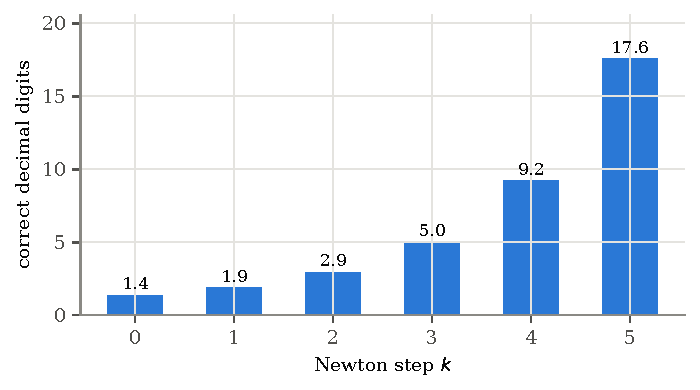
\includegraphics[width=0.7\textwidth]{figures/newton_convergence.pdf}
\caption{Correct digits of $1/7$ after each Newton step, starting from $0.1$. Each step
roughly doubles them. Computed with exact fractions by \file{figures/make\_figures.py}.}
\label{fig:newton}
\end{figure}

\subsection{Why the whole computation costs about two multiplications}

Because accuracy doubles each step, the early steps only need low precision. To get $n$
limbs, the last step works with $n$ limbs, the one before with $n/2$, the one before that
with $n/4$, and so on. The costs form a halving series: $\M(n) + \M(n/2) + \M(n/4) + \dots$,
which adds up to less than $2\,\M(n)$ for each multiplication in a step. Getting the
reciprocal costs a small constant number of full-size multiplications, not $\log n$ of them.

\subsection{In integers}

The library never uses fractions. For an $n$-limb normalized divisor $D$ it computes an
integer $R$ approximating $B^{2n}/D$, which is $1/D$ ``scaled up'' by $B^{2n}$. BigMath's
\code{ApproxReciprocal} guarantees
\[
0 \le \floor{B^{2n}/D} - R \le 3 ,
\]
that is, $R$ is never too large and at most 3 too small.

Two details make this work cheaply:

\begin{itemize}
  \item \textbf{A guarded precision schedule.} A Newton step on a $p$-limb estimate gives
        \emph{almost} $2p$ limbs, a few bits short. If each step asks for exactly double, the
        shortfall doubles too, and the final result can be off by a lot. BigMath instead works
        out the precisions \emph{backwards} from $n$: each earlier precision is
        $\ceil{(p + 2)/2}$, so each step has two guard limbs to spare. The first estimate is an
        exact reciprocal of the divisor's top (at most 32) limbs, computed with long division.
        This removed an extra full-size ``cleanup'' iteration the old code needed.
  \item \textbf{Only the new limbs are computed.} A step can be rewritten as
        ``old value, shifted, plus a correction'', where the correction depends on a small error
        term. Only the top limbs of the correction product are needed, so the step multiplies
        shorter numbers than the textbook formula.
\end{itemize}

\subsection{From the reciprocal to the quotient}

With $R \approx B^{2n}/D$ in hand, dividing a chunk of at most $2n$ limbs is:

\begin{enumerate}
  \item \textbf{Estimate}: $\hat q = \floor{\text{(top limbs of the chunk)} \times R / B^{2n}}$,
        one multiplication. Only the top $n+1$ limbs of the chunk can affect $\hat q$ (the rest
        contributes less than one unit), so only those are multiplied.
  \item \textbf{Remainder}: $r = \text{chunk} - \hat q \cdot D$, a second multiplication.
  \item \textbf{Fix up}: $\hat q$ is at most a few units too small; while $r \ge D$, subtract $D$
        and increase $\hat q$.
\end{enumerate}

\begin{figure}[ht]
\centering
\begin{tikzpicture}[x=1cm,y=1cm]
  \fill[sBlue!25,draw=ink2] (0,0) rectangle (2.6,0.6) node[midway,font=\footnotesize] {leading chunk};
  \foreach \k in {1,2,3} \fill[sBlue!12,draw=ink2] ({2.6+(\k-1)*2.2},0) rectangle +(2.2,0.6) node[midway,font=\footnotesize] {block \k};
  \node[lbl,anchor=east] at (-0.1,0.3) {dividend};
  \draw[decorate,decoration={brace,amplitude=4pt,mirror}] (2.6,-0.1) -- (4.8,-0.1) node[midway,below=4pt,lbl] {$n$ limbs};
  \draw[arr] (1.3,-0.25) to[bend right=25] node[below,lbl] {remainder carries into next block} (3.7,-0.95);
  \node[box,fill=sOrange!20] at (11.5,0.3) {$R \approx B^{2n}/D$\\computed once};
\end{tikzpicture}
\caption{Blockwise Newton division: the reciprocal is computed once and reused for every
block of the dividend. Each block's remainder becomes the top of the next block.}
\end{figure}

For a long dividend the library processes it in blocks of $n$ limbs from the top, carrying
each remainder into the next block, and reusing the same $R$ throughout. The cost is the
reciprocal (a few $\M(n)$) plus about two $\M(n)$ per block. The more blocks there are, the
more the reciprocal is amortized: this is why Newton wins for lopsided divisions.

\subsection{The wrap-around remainder}
\label{sec:wrap}

Step 2 computes the full product $\hat q \cdot D$, about $2n$ limbs, only to subtract it from
the chunk and get a remainder that is known to be small (less than a few times $D$, so about
$n + 1$ limbs). Most of the product cancels.

Here the wrap-around of \cref{ch:ntt} becomes useful. A cyclic transform of length $L$
computes the product modulo $B^L - 1$ at about half the cost of the full product. If
$L \ge n + 2$, the remainder is small enough to be recovered exactly from
$(\text{chunk} - \hat q D) \bmod (B^L - 1)$, and whether it is negative can be read from its
size. The same trick computes the error term inside the reciprocal's Newton steps. Each of
these changes (wrapped remainder, wrapped reciprocal error, multiplying only the chunk's top
limbs) cut 10--25\% from large one-off divisions; together they took a 5-million by
1-million-digit division from 206\,ms to 111\,ms.

\subsection{Small leading blocks go to long division}

A dividend of exactly $k \cdot n$ limbs often gains one limb when it is normalized. That
leading block then has a one-limb quotient, but a full Newton chunk would cost two $n$-limb
multiplications to produce it. Leading blocks with at most 32 quotient limbs
(\code{BIGMATH\_NEWTON\_SCHOOLBOOK\_HEAD}) go to Algorithm D instead, which costs about 1.3\,ns
per divisor limb per quotient limb against 60--75\,ns for a chunk.

\begin{pitfall}
If a Newton quotient estimate is ever off by more than the fix-up loop allows, the code
falls back to long division. The answer is still correct, just quadratic, so nothing in the
correctness tests would notice. Once, a too-tight error bound in the reciprocal triggered
this fallback on every divide inside \code{ToString}, an 8-fold slowdown that was invisible
except in timings. \code{NewtonDivision::FallbackCount()} now counts fallbacks and the unit
tests assert it stays at zero.
\end{pitfall}

\section{Short quotients: only the top limbs matter}
\label{sec:toplimbs}

Suppose $a$ has 10\,010 limbs and $b$ has 10\,000. The quotient has only 11 limbs. Does
computing it really need all 20\,010 input limbs? No. A short quotient is decided by the
leading limbs of the operands; the rest can only move it by a tiny fraction.

\begin{example}[: estimating a quotient from the leading digits]
$a = 98\,765\,432\,198$ and $b = 123\,456\,789$. The quotient has about $11 - 9 + 1 = 3$ digits.
Keep the quotient length plus two guard digits of $b$, that is 4 digits, and the matching
digits of $a$:
\[
a' = 987\,654, \qquad b' = 1234, \qquad a' \div b' = 800 \text{ remainder } 454 .
\]
The true answer: $123\,456\,789 \times 800 = 98\,765\,431\,200$, remainder $998$. So $q = 800$,
found from a 6-digit by 4-digit division.
\end{example}

BigMath uses this in two places.

\paragraph{Quotient only (\code{a / b}).} When you ask only for the quotient and it is shorter
than the divisor, the dispatcher keeps $t = \delta + 4$ top limbs of $b$ (where
$\delta = n_a - n_b$) and the matching top limbs of $a$, and divides those. A short argument
shows the true quotient is either $q'$ or $q' - 1$, and it is $q'$ whenever the top remainder
$r'$ is at least $B^{\delta + 2}$, which for random inputs fails with probability about
$2^{-128}$. Only in that rare case (or when $a$ is an exact multiple of $b$, which always lands
there) is one $\delta \times n_b$ product computed to decide. The work drops from
$\delta \times n_b$ to a $(2\delta + 4)$-by-$(\delta + 4)$ division.

\begin{center}
\small
\begin{tabular}{rrrrr}
\toprule
divisor limbs & quotient limbs & before (\textmu s) & now (\textmu s) & GMP \code{mpz\_tdiv\_q} \\
\midrule
512 & 11 & 3.56 & 0.29 & 0.17 \\
1024 & 103 & 44.0 & 7.27 & 3.97 \\
4096 & 83 & 89.7 & 4.94 & 2.74 \\
16384 & 329 & 332 & 47.3 & 25.7 \\
\bottomrule
\end{tabular}
\end{center}

\paragraph{Quotient-sized division (with remainder).} When the remainder is also wanted and the
quotient is long (at least 3072 limbs) but still shorter than the divisor,
\code{QuotientSizedDivision} divides the operand tops (with Newton for large sizes), then
computes the remainder with one $\delta \times n_b$ multiplication and a few corrections. Its
cost scales with the \emph{quotient}, not the divisor.

\section{Reusing a divisor}
\label{sec:cached}

The reciprocal is the expensive part of Newton division, and it depends only on the divisor.
If you divide many numbers by the same divisor, compute it once:

\begin{lstlisting}
#include "biginteger/ops/Division.h"
CachedDivision div = CacheDivision(modulus);   // computes and stores the reciprocal
for (auto const &x : values) {
    auto [q, r] = div.DivideAndRemainder(x);    // reuses it every time
}
\end{lstlisting}

For five divisions by the same large divisor, the cached form measured 27--31 times faster
than five independent divisions (12--25 times including the one-time setup). Decimal printing
(\cref{ch:conv}) is built on exactly this.
